\section{Naravna in cela števila, izrazi, enačbe in neenačbe}

\begin{frame}
    \sectionpage
\end{frame}

\begin{frame}
    \tableofcontents[currentsection, hideothersubsections]
\end{frame}
        
    \subsection{Naravna in cela števila}

        \begin{frame}
            \frametitle{Naravna števila}

            \textbf{Množica naravnih števil}: 
                \begin{alertblock}{}
                    \centering\boldmath
                    $\mathbb{N}=\{1, 2, 3, 4, \ldots\}$
                \end{alertblock}

            Naravna števila so števila s katerimi štejemo.
            
            \medskip
            Naravna števila lahko predstavimo s \textbf{točko} na \textbf{številski premici}.
                \begin{figure}
                    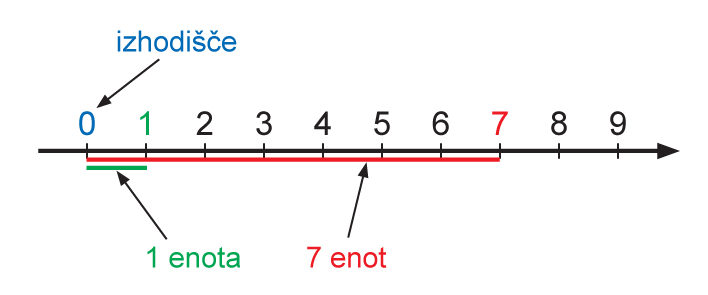
\includegraphics[scale=0.65]{Slike in skice/Stevilska_premica.png}
                \end{figure}
        \end{frame}

        \begin{frame}
            Množico naravnih števil definirajo \textbf{Peanovi aksiomi}:
            \begin{itemize}
                \item Vsako naravno število ($n$) ima svojega naslednika ($n+1$).
                \item Število $1$ ni naslednik nobenega naravnega števila.
                \item Različni naravni števili imata različna naslednika: ($n+1 \neq m+1;\quad n \neq m$).
                \item Če neka trditev velja za vsako naravno število in tudi za njegovega naslednika, velja za vsa naravna števila - princip popolne indukcije.
            \end{itemize}
            
            \bigskip
            V množici $\mathbb{N}$ sta definirani notranji operaciji: \textbf{seštevanje} in \textbf{množenje}.
        \end{frame}

        \begin{frame}
            \textbf{\large{Seštevanje}}
            
            \bigskip
            Poljubnima naravnima številoma $a$ in $b$ priredimo \textbf{vsoto} $\mathbf{a+b}$.
            
            \bigskip
            Vsota naravnih števil je naravno število: $a, b \in \mathbb{N} \Rightarrow a+b \in \mathbb{N}$.
            
            \bigskip
            Lastnosti:
            \begin{itemize}
                \item \textit{\textbf{komutativnost}} členov/zakon o zamenjavi členov: $a+b = b+a$.
                \item \textit{\textbf{asociativnost}} členov/zakon o združevanju členov: $(a+b)+c = a+(b+c)$.
            \end{itemize}

        \end{frame}

        \begin{frame}
            \textbf{\large{Množenje}}
            
            \bigskip
            Poljubnima naravnima številoma $a$ in $b$ priredimo \textbf{produkt} $\mathbf{a\cdot b}$.
            
            \bigskip
            Produkt naravnih števil je naravno število: $a, b \in \mathbb{N} \Rightarrow a \cdot b \in \mathbb{N}$.            

            \bigskip
            Lastnosti:
            \begin{itemize}
                \item \textit{\textbf{komutativnost}} faktorjev/zakon o zamenjavi faktorjev: $a \cdot b = b \cdot a$.
                \item \textit{\textbf{asociativnost}} faktorjev/zakon o združevanju faktorjev: $(a \cdot b) \cdot c = a \cdot (b \cdot c)$.
                \item \textit{\textbf{distributivnost}}/zakon o razčlenjevanju: $a \cdot (b+c) = a \cdot b + a \cdot c$.
                \item zakon o nevtralnem elementu: $a \cdot 1 = a$.
            \end{itemize}

        \end{frame}

        \begin{frame}
            \frametitle{Cela števila}
        \end{frame}

    \subsection{Računanje z naravnimi in celimi števili}

        \begin{frame}
            \frametitle{Računanje z naravnimi in celimi števili}
        \end{frame}

    \subsection{Izraz, enačba, neenačba}

        \begin{frame}
            \frametitle{Izraz, enačba, neenačba}
        \end{frame}

    \subsection{Računanje s potencami z naravnimi eksponenti}

        \begin{frame}
            \frametitle{Računanje s potencami z naravnimi eksponenti}
        \end{frame}

    \subsection{Razčlenjevanje izrazov}

        \begin{frame}
            \frametitle{Razčlenjevanje izrazov}
        \end{frame}

    \subsection{Razstavljanje izrazov v množici $\mathbb{Z}$}

        \begin{frame}
            \frametitle{Razstavljanje izrazov v množici $\mathbb{Z}$}
        \end{frame}

    \subsection{Reševanje linearnih in razcepnih enačb v množici $\mathbb{Z}$}

        \begin{frame}
            \frametitle{Reševanje linearnih in razcepnih enačb v množici $\mathbb{Z}$}
        \end{frame}

    \subsection{Reševanje linearnih neenačb v množici $\mathbb{Z}$}

        \begin{frame}
            \frametitle{Reševanje linearnih neenačb v množici $\mathbb{Z}$}
        \end{frame}
